%%%%%%%%%%%%%%%%%%%%%%%%%%%%%%%%%%%%%%%%%%%%%%%%%%%%%%%%%%%%%%%%%%%%%%%%%%%%%
%
%  System        : 
%  Module        : 
%  Object Name   : $RCSfile$
%  Revision      : $Revision$
%  Date          : $Date$
%  Author        : $Author$
%  Created By    : Robert Heller
%  Created       : Mon Jul 15 17:34:14 2019
%  Last Modified : <200211.1349>
%
%  Description 
%
%  Notes
%
%  History
% 
%%%%%%%%%%%%%%%%%%%%%%%%%%%%%%%%%%%%%%%%%%%%%%%%%%%%%%%%%%%%%%%%%%%%%%%%%%%%%
%
%    Copyright (C) 2019  Robert Heller D/B/A Deepwoods Software
%			51 Locke Hill Road
%			Wendell, MA 01379-9728
%
%    This program is free software; you can redistribute it and/or modify
%    it under the terms of the GNU General Public License as published by
%    the Free Software Foundation; either version 2 of the License, or
%    (at your option) any later version.
%
%    This program is distributed in the hope that it will be useful,
%    but WITHOUT ANY WARRANTY; without even the implied warranty of
%    MERCHANTABILITY or FITNESS FOR A PARTICULAR PURPOSE.  See the
%    GNU General Public License for more details.
%
%    You should have received a copy of the GNU General Public License
%    along with this program; if not, write to the Free Software
%    Foundation, Inc., 675 Mass Ave, Cambridge, MA 02139, USA.
%
% 
%
%%%%%%%%%%%%%%%%%%%%%%%%%%%%%%%%%%%%%%%%%%%%%%%%%%%%%%%%%%%%%%%%%%%%%%%%%%%%%

\chapter{LCCCANCape: LCC CAN Tranceiver Cape}

\section{GPIO Pins Used and stacking restrictions.}

This board uses two pins on header P9: 24 and 26 in pin mux mode2, which makes 
pin 24 Can1 RX, and pin 26 Can1 TX.  Only one of these capes can be on any 
Beagle Bone Black.


\section{Circuit Description}

\begin{figure}[hbpt]\begin{centering}%                                         
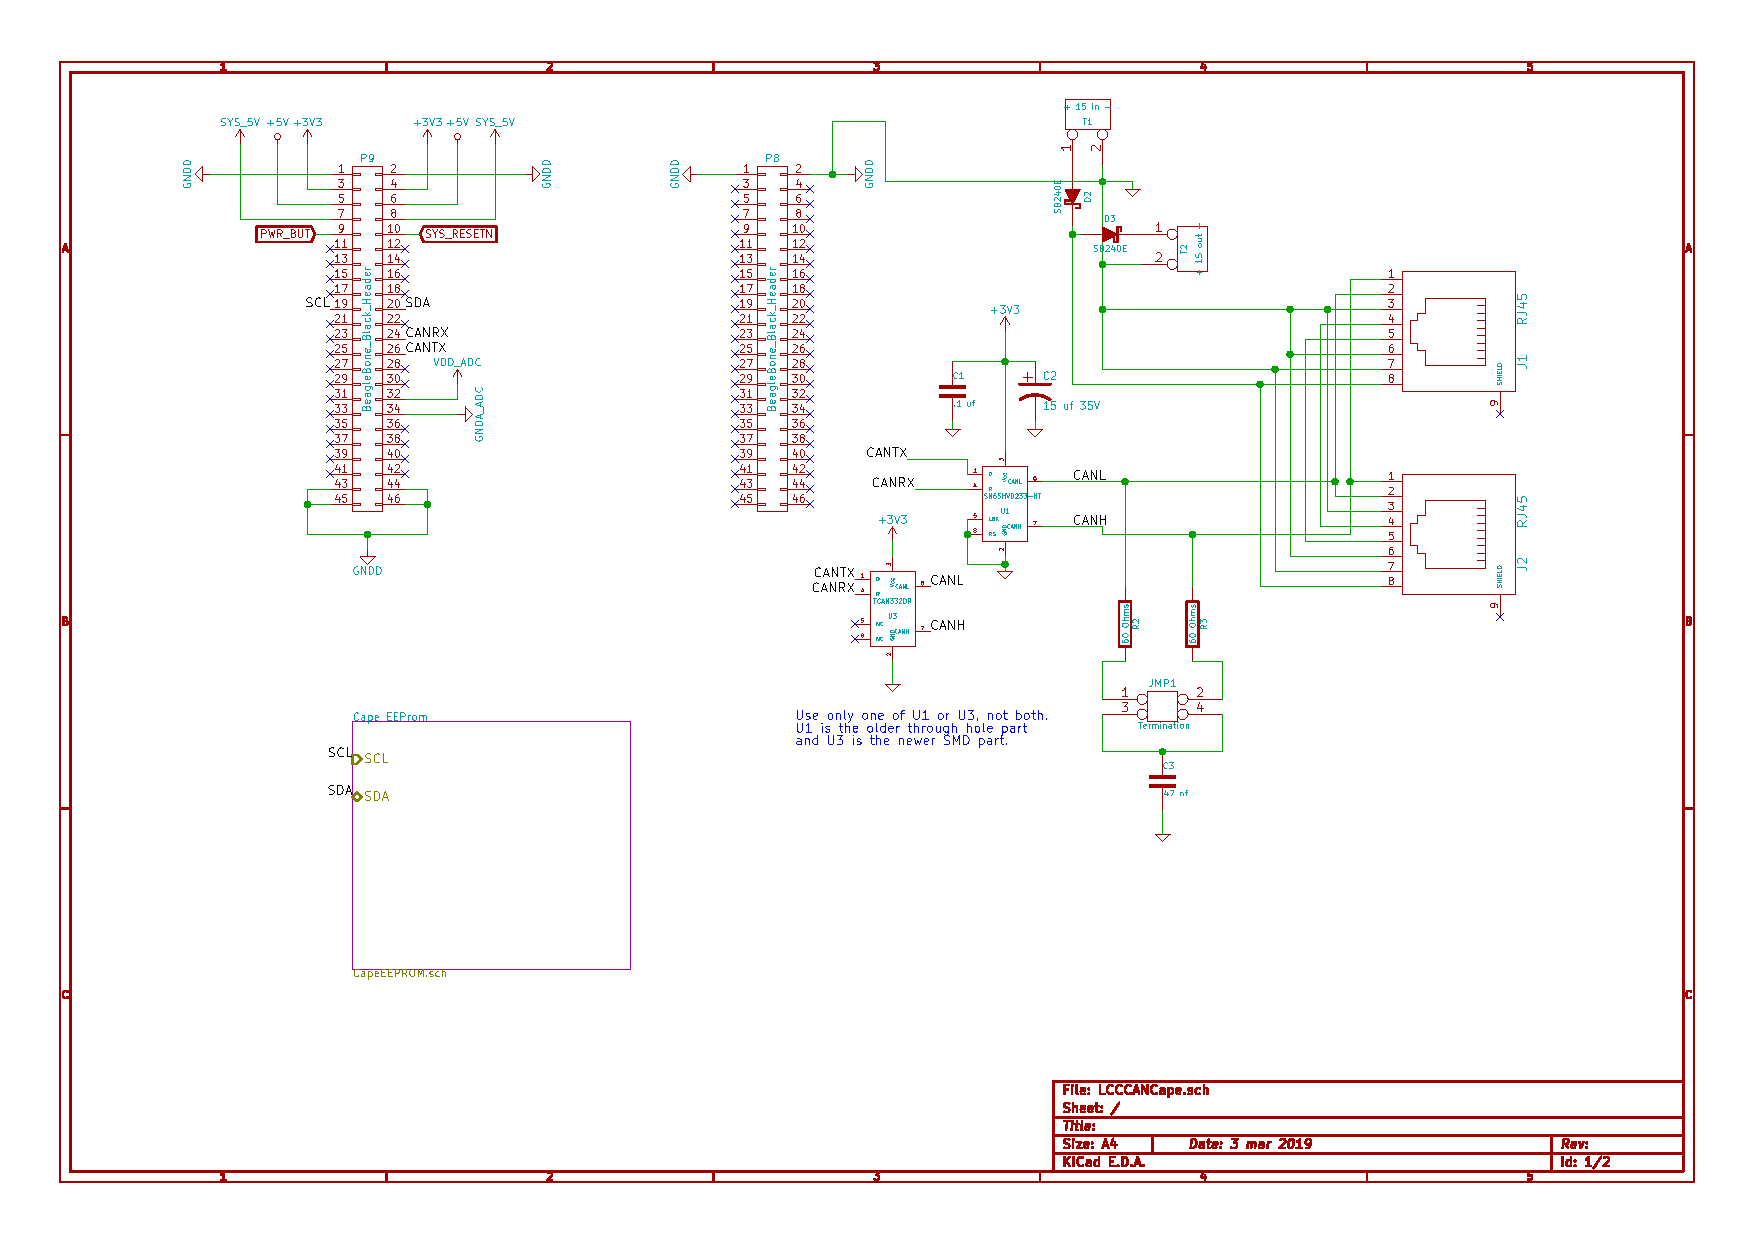
\includegraphics[width=5in]{LCCCANCape-1.pdf}                               
\caption{Circuit Diagram of the LCCCANCape}                               
\end{centering}\end{figure}                                                    
This circuit contains two sectins.  There is the transciever section, which 
includes the transciver itself, the termination block, the two RJ45 jacks, and 
two terminal blocks for injecting and tapping into the power carried in the 
CAT 5 cable.  Power is not used to power the Beagle Bone Black.  The other 
section is the Cape EErom circuit.  The Cape EEProm contains         
information about the cape and the name and version of the overlay that needs  
to be loaded by uBoot.  

\clearpage

\section{Parts List}

\begin{table}[htdp]
\begin{centering}\begin{tabular}{|l|l|p{1in}|l|}
\hline
Value&Quantity&References&Mouser Part Number \\
\hline
.1 uf&1&C8&581-SR201C104KARTR1 \\
\hline
WP 1 0&1&P2&649-67996-406HLF \\
\hline
5.6K Ohms&2&R3 R4&603-CFR-25JR-525K6 \\
\hline
4.75K Ohms&3&R5 R6 R7&603-CFR-25JR-524K7 \\
\hline
10K Ohms&1&R8&603-CFR-25JR-5210K \\
\hline
CAT24C256W&1&U9&698-CAT24C256WI-GT3 \\
\hline
.1 uf&1&C1&21RZ310-RC \\
\hline
15 uf 63V&1&C2&710-860080773002 \\
\hline
47 nf&1&C3&75-1C10Z5U473M050B \\
\hline
SB240E&2&D1 D2&625-SB240-E3 \\
\hline
RJ45&2&J1 J2&710-615008144221 \\
\hline
Termination&1&JP1&649-67997-404HLF \\
\hline
60 Ohms&2&R1 R2&71-RN60C60R0B/R \\
\hline
+ 15 in -;+ 15 out -&2&T1 T2&651-1725656 \\
\hline
TCAN332DR&1&U1&595-TCAN332DR \\
\hline
SN65HVD233-HT&1&U2&595-SN65HVD233SJD \\
\hline
BeagleBone\_Black\_Header&2&''P8 P9''&200-ESQ12314GD \\
\hline
\end{tabular}
\caption{Parts list for LCCCANCape board.}
\end{centering}\end{table}\footnote{Mouser Project links: 
\url{http://www.mouser.com/ProjectManager/ProjectDetail.aspx?AccessID=ae58a2d985},
\url{http://www.mouser.com/ProjectManager/ProjectDetail.aspx?AccessID=522a1259b2}.}


The only parts that might be substituted are P8 and P9 (the Beagle Bone Black
Headers). The parts listed are for the stacking headers for the Beagle Bone
Black Headers. Feel free to select a non-stacking header for the Beagle Bone
Black Headers.


\section{Circuit Board Layout}

\begin{figure}[hbpt]\begin{centering}%
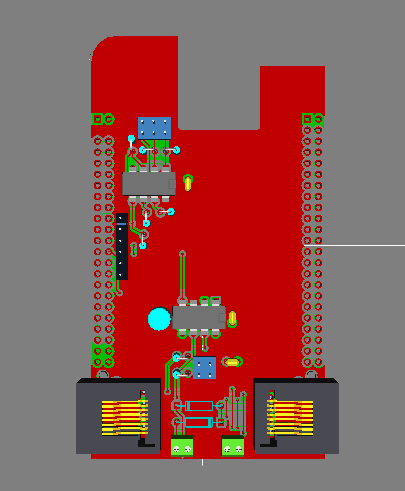
\includegraphics[height=7in]{LCCCANCape3DTop.png}
\caption{3D rendering of the LCCCANCape board}
\end{centering}\end{figure}
\begin{figure}[hbpt]\begin{centering}%
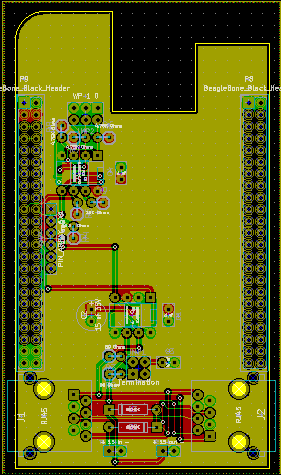
\includegraphics[height=7in]{LCCCANCape.png}
\caption{Fabrication image of the LCCCANCape board}
\end{centering}\end{figure}
Board assembly is straight forward. You need to be careful orienting the ICs
and the electrolytic capacitor.


\section{Downloadables and Software Support}

Full design information is available on GitHub here:
\url{https://github.com/RobertPHeller/RPi-RRCircuits/tree/master/LCCCANCape}.

This board is supported by both the Model Railroad System 
(\url{https://github.com/RobertPHeller/ModelRRSystem}) and the OpenMRN 
(\url{https://github.com/bakerstu/openmrn}).
